\documentclass[%handout,
	sans,			% use sans-serif font
	%serif,			% use serif-font
	mathsans,		% set mathtext to sans-serif
	%mathserif,		% set mathtext to serif
	%10pt,
	10pt,
	%12pt,
	t		% add text at the top border of slide
	slidescentered,% center text on slide
	%draft,			% compile as draft version
	%notes,			% include nodes in slides
	%compress		% compress navigation bar
]{beamer}


\usetheme{lmtslides}
\setlang{en}
\usepackage{eso-pic}
\usepackage{graphicx}
%\usepackage[pdftex]{color}
\usepackage{times}
\usepackage[utf8x]{inputenc}
\usepackage[amssymb]{SIunits}
\usepackage{amsmath,amssymb}
\usepackage{booktabs}
\usepackage{colortbl}
\usepackage{url}
\usepackage{csquotes}

\usepackage{default}
\usepackage{hyperref}

\usepackage{mathptmx}
\DeclareMathAlphabet{\mathcal}{OMS}{cmsy}{}{n}

\renewcommand*\sfdefault{uop}
\usepackage[T1]{fontenc}

\graphicspath{{figures/}}


\newcommand{\RR}{\mathbb{R}}
\newcommand{\NN}{\mathbb{N}}
\newcommand{\QQ}{\mathbb{Q}}
\newcommand{\sturm}{\texttt{sturm}}
\newcommand{\lem}{\textbf{lemma}}
\newcommand{\card}{\textrm{card}}
\newcommand{\real}{\textrm{real}}


% MODIFY THESE ACCORDINGLY! ---
\title[asdf]{A Formalisation of Sturm's Theorem\\in Isabelle/HOL}
\subtitle{}
\type{IDP Talk}
\author{Manuel Eberl}
\email{eberlm@in.tum.de}
\date{12 December 2013} % TODO
%------------------------------


%%%%%%%%%%%%%%%%%%%%%%%%%%
\begin{document}

\AddToShipoutPicture{\TitlePicture}
\maketitle
\ClearShipoutPicture
\AddToShipoutPicture{\BackgroundPicture}

\begin{frame}{Motivation}
\begin{description}
\item[We have:] a polynomial with real coefficients
\pause\item[We want:] the number of real roots in a specific interval
\end{description}
\end{frame}

\begin{frame}{Motivation}
\vspace*{1.65mm}
\begin{description}
\item[We have:] a polynomial with $\overbrace{\text{\color{red}real\ coefficients}}^{\text{not\ really}}$
\vspace*{-0.05mm}
\item[We want:] the number of real roots in a specific interval
\end{description}
\vspace{5mm}
\pause
For \enquote{real} computations: restricted to appropriate subset of $\RR$, such as $\QQ$.
\end{frame}

\begin{frame}{Motivation}
The solution: \emph{Sturm's Theorem}\\[2mm]

Provides a method for counting real roots \emph{algorithmically}.\\[10mm]

$\Longrightarrow$ Let's formalise it in Isabelle/HOL
\end{frame}

\begin{frame}{Notation}
\emph{Sign changes:} $\sigma(P_0,\ldots,P_{n-1}; x)$ denotes denotes the number of sign changes in the sequence $P_0(x), \ldots, P_{n-1}(x)$\\[2mm]
For the functionally inclined:\vskip-6mm
$$\sigma(ps; x) = (\mathrm{length} \circ \mathrm{remdups\_adj} \circ \mathrm{filter}\ (\neq 0) \circ \mathrm{map}\ (\lambda p.\ p(x)))\ ps\ -\ 1$$
\end{frame}

\begin{frame}{Sturm's Theorem}
Sturm's Theorem: \textit{Let $P$ be a real polynomial and $P_0, \ldots, P_{n-1}$ a Sturm sequence of $P$. Then
$$\sigma(P_0, \ldots, P_{n-1}; a) - \sigma(P_0, \ldots, P_{n-1}; b)$$
is the number of real roots of $P$ in the interval $(a; b]$.}
\end{frame}

\begin{frame}{Sturm sequence}
But what is a Sturm sequence of $P$?\\
A (reasonably) general definition:\\
\begin{itemize}
\item $P_0 = P$
\item $P_0$ and $P_1$ have no common roots
\item $P_{n-1}$ (last element) does not change its sign
\item if $x_0$ is root of $P_0$: $P_0P_1(x)<0$ in some left-NH and $P_0P_1(x)>0$ in some right-NH of $x_0$
\item if $x_0$ is root of another $P_i$: $P_{i-1}P_{i+1}(x_0) < 0$
\end{itemize}
\end{frame}

\begin{frame}{Assessment}
\begin{description}
\item[The good news:]\ \\formalisation of real analysis, polynomials, algebra already exists
\pause\item[The bad news:]\ \\no formalisation of limits of polynomials, very little on divisibility
\pause\item[The ugly news:]\ \\textbook proofs of \emph{Sturm's theorem} are \emph{extremely} informal proof sketchs at best
\end{description}
\end{frame}

\begin{frame}{Proving Sturm's Theorem}
Assume we already have a Sturm chain. Why does it count roots?\\
Follow $x \mapsto \sigma(P_0, \ldots, P_{n-1}; x)$ passing over $\RR$. Obviously, it can only change at $x_0$ if one of the $P_i$ has a root at $x_0$
\begin{itemize}
\item if $P_i \neq P_0$ has $x_0$ as a root, $P_{i-1}P_{i+1}(x_0) < 0$\\
$\Rightarrow$ signs of $P_{i-1}$, $P_{i+1}$ are $\neq 0$, opposite, constant in NH of $x_0$\\
$\Rightarrow$ signs $[1,\, \_\,, -1]$ or $[-1,\, \_\,, 1]$ in the entire NH, i.e. one sign change\\
$\Rightarrow$ total number of sign changes not influenced\\[1mm]
\item if $P_0$ has $x_0$ as root, $P_0P_1(x_0) < 0$ in left-NH of $x_0$, $>0$ in right-NH\\
$\Rightarrow$ signs are different left of $x_0$ and the same right of $x_0$\\
$\Rightarrow$ total number of sign changes decreases by one
\end{itemize}
\end{frame}

\begin{frame}{Proving Sturm's Theorem}
Formal proof: a lot of induction on the sequences and number of roots\\[2mm]
$\Longrightarrow$ messy and not terribly interesting
\end{frame}

\begin{frame}{Construction Sturm sequences}
Canonical construction for $P$ with no multiple roots (i.e. $\mathrm{gcd}(P,P') = 1$):
$$P_i = \begin{cases}
P & \mathrm{for}\ i = 0\\
P' & \mathrm{for}\ i = 1\\
-(P_{i-2}\ \mathrm{mod}\ P_{i-1}) & \mathrm{otherwise}
\end{cases}$$
\end{frame}

\begin{frame}{Construction Sturm sequences}
Why does it work? Nonobvious parts:\\[3mm]

If $x_0$ is root of $P_0 = P$: $PP'(x_0) < 0$ in left-NH and $PP'(x_0) > 0$ in right-NH\\
-- pick neighbourhood without roots of $P_0$ and $P_1$ (except for $x_0$),\\
\hskip3mm apply mean value theorem\\[3mm]

If $x_0$ is root of another $P_i$: $P_{i-1}P_{i+1}(x_0) < 0$ in some NH of $x_0$\\
-- by construction, $P_{i-1} = Q\cdot P_i - P_{i+1}$ for some $Q\in\RR[X]$\\
\hskip3mm$\Longrightarrow$ $P_{i-1}(x_0) = -P_{i+1}(x_0)$\\
\hskip3mm also: $P_{i-1}(x_0)\neq 0$ since $\mathrm{gcd}(P_{i-1}, P_i) = \mathrm{gcd}(P_0,P_1) = 1$
\end{frame}

\begin{frame}{Construction Sturm sequences}
In case of multiple roots: Let $D := \mathrm{gcd}(P,P')$. Then:
\begin{description}
\item[The obvious way:]\ \\
\begin{itemize}
\item compute canonical Sturm chain of $P / D$\\ (\enquote{divide out} multiple roots)
\end{itemize}
\item[The clever way:]\ \\
\begin{itemize}
\item we can compute the canonical Sturm chain of $P$ and divide by $D$ afterwards
\item but: if $D(x)\neq 0$, dividing by $D$ does not change the number of sign changes at $x$
\item $\Longrightarrow$ unless the interval bounds are multiple roots, we can use the canonical construction without changes
\end{itemize}
\end{description}
\end{frame}

\begin{frame}{Making a decision procedure}
\textit{count\_roots\_between\ p\ a\ b}: picks the most efficient Sturm chain construction and:
$$\textit{count\_roots\_between}\ p\ a\ b\ \ =\ \ |\{x.\ a < x\ \wedge\ x \leq b\ \wedge\ p(x) = 0\}|$$\vskip2mm

Some fluff:
\begin{itemize}
\item case distinctions allow arbitrary combination og $\leq$ and $<$ in bounds
\item \enquote{limit signs} allow infinite bounds
\end{itemize}
In summary: we can count roots in any open/halfopen/closed, bounded/unbounded real interval
\end{frame}

\begin{frame}{Making a decision procedure}
Some more fluff:
\begin{itemize}
\item and/or: count $x$ with $$P(x)=0\ \wedge\ Q(x)=0\hskip5mm\mathrm{or}\hskip5mm P(x)=0\ \vee\ Q(x)=0$$
\item $\forall$-inequalities: $$\forall x.\ P(x) \neq Q(x)\ \wedge\ R(x) \neq S(x)\ \vee\ T(x)\neq U(x)$$
\item $\forall$ with $<$ and $>$: $$\forall x.\ P(x) < Q(x)\ \wedge\ R(x) > S(x)\ \vee\ T(x)\neq U(x)$$
\end{itemize}
\end{frame}

\begin{frame}{\hskip-2mm Making a decision procedure}
\hskip-2mm Examples:
\begin{align*}
&\hskip-2mm\scriptstyle
\lem\ "\card\ \{x::\real.\ (x\, -\, 1)^2\, *\, (x\, +\, 1)\ =\ 0\}\ =\ 2"\ \textrm{\textbf{by}\ sturm}\\[2mm]
&\hskip-2mm\scriptstyle\textbf{lemma}\ "\mathrm{card}\ \{x::\mathrm{real}.\ -0.010831\, <\, x\ \wedge\ x\, <\, 0.010831\ \wedge\\
&\hskip-2mm\scriptstyle\hskip20mm \mathrm{poly}\ [:\,0,\  -17/2097152,\  -49/16777216,\  1/6,\  1/24,\  1/120\,:]\ x\ =\ 0\}\  =\  3"\ \textrm{\textbf{by}\ sturm}\\[2mm]
&\hskip-2mm\scriptstyle\lem\ "\card\ \{x::\real.\ x^3\, +\, x\ =\ 2\,*\,x^2\ \wedge\ x^3\,-\,6*x^2\,+\,11*x\ =\ 6\}\  =\  1"\ \textrm{\textbf{by}\ sturm}\\[2mm]
&\hskip-2mm\scriptstyle\lem\ "(x::\real)^2\,+\,1\ >\ 0"\ \textrm{\textbf{by}\ sturm}
\end{align*}
\end{frame}

\begin{frame}{Size of the formalisation}
3725 LOC in total, 185 of that ML, the rest Isabelle
\begin{center}
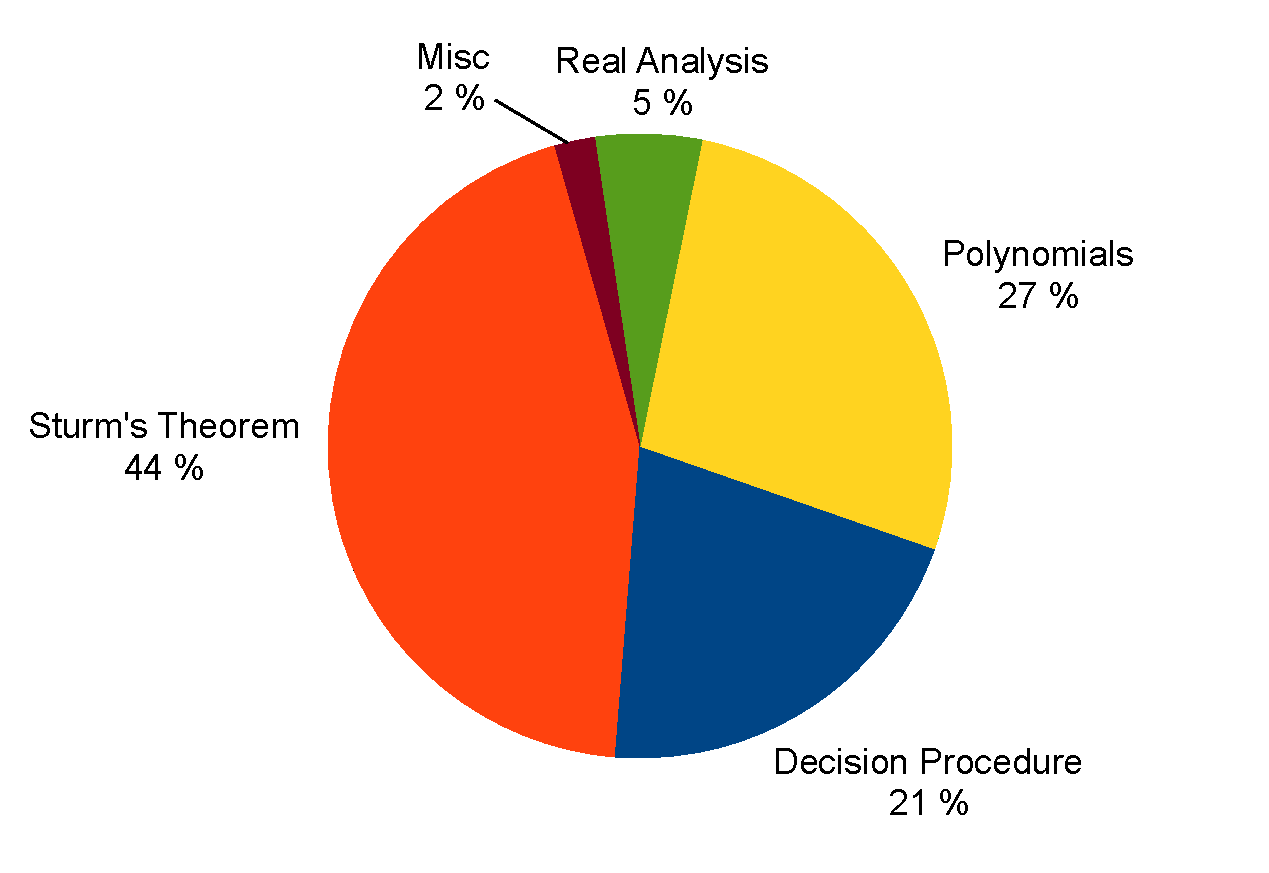
\includegraphics[width=8cm]{plot.pdf}
\end{center}
\end{frame}

\end{document}
